\scanpage{96}

En vertu du Cor. au lemme 1, on est
ramené à prouver que en tt pt
\unsure{de} $x$ de $Y$ de codim 1 dans $Y$, \deleted{\unsure{on}}
$X'$ est \deleted{\unsure{non ramifié}} étale sur $X$ en les
$g(x)$. [N.B. Comme $X\unsure{-|\to}Y$ est
simple de dim relative 1, on notera
que $g(Y)$ est \deleted{défini loc. par} loc. un
diviseur de Cartier]. On est ainsi
ramené au cas où $Y$ est \deleted{le} spectre
d'un anneau de val. discrète, et \deleted{\unsure{qui}} on
est alors ramené [\unsure{en} examinant $\mathscr O_{X,g(x)}$]

% slanted
\margin{On a laissé tomber les conditions ``quotient d'un régulier'', c'est \unsure{loisible} en se ramenant aux alg. de type fini sur $\mathbb Z$\ldots}

\uline{Lemme 3} \quad Soit $A$ un anneau local
\uline{régulier} de dim $2$, $(x,y)$ un syst. régulier
de paramètres de $A$, $B$ une
``extension'' normale de $A$,
\deleted{\unsure{non ramifiée au pt}} \inserted{telle que}
\unsure{galoisienne|génériquemt}, (i) \deleted{de} groupe de Galois $\Gamma$
d'ordre premier à la car. résiduelle de $A$,
et telle que \deleted{\unsure{$B$ sur|$B\to$}} (ii) l'ens de ramification
de $B$ soit contenu dans $V(x)$ (iii)
le rev. se décompose complètemt en \deleted{$V(y)$}
le pt maximal $\unsure{y|\eta}$ de $V(y)$.

\figure{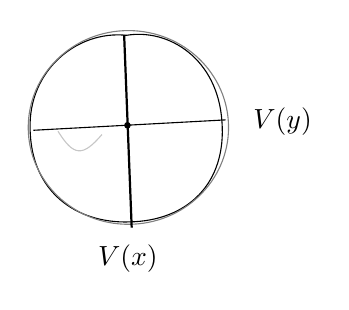
\begin{tikzpicture}[x=.6cm,y=.6cm]
\draw (0,1.95) .. controls (-1.05,2.06) and (-2.08,1.2) .. (-2.04,-.03) .. controls (-2.02,-1.38) and (-1.05,-2.03) .. (.05,-2) .. controls (1.31,-1.98) and (2.12,-1.17) .. (2.02,.13) .. controls (1.93,1.45) and (.9,2.1) .. (0,1.95);
\draw[thin,gray] (.04,0) ellipse (2.12 and 2.05);
\draw[thin,gray!45] (-1.45,-.08)..controls(-1.12,-.61)and(-.93,-.63)..(-.52,-.15);
\draw[line width=.8pt] (-.05,1.96)--(.11,-2.12);
\draw (-1.97,-.06)--(2.1,.16); \fill (.02,.045) circle (.07);
\node[right] at (2.48,.13) {$V(y)$}; \node[below] at (.03,-2.28) {$V(x)$};
\end{tikzpicture}}

% archive sheet number: 95
